% ------------------------------------------------------------
% Global distribution graph dimensions
% ------------------------------------------------------------
\newlength{\DistributionGraphWidth}
\newlength{\DistributionGraphHeight}

\setlength{\DistributionGraphWidth}{0.8\textwidth}
\setlength{\DistributionGraphHeight}{6cm}


% ==========================================================================
% 1. NORMAL DISTRIBUTION PDF GRAPH
% X ~ N(mu,sigma^2)
% X-axis shows only numerical values.
% ==========================================================================

\newcommand{\CNormalPDFGraph}[2]{%
	\pgfmathsetmacro{\MuMinusThreeSigma}{#1-3*#2}%
	\pgfmathsetmacro{\MuMinusTwoSigma}{#1-2*#2}%
	\pgfmathsetmacro{\MuMinusSigma}{#1-#2}%
	\pgfmathsetmacro{\Mean}{#1}%
	\pgfmathsetmacro{\MuPlusSigma}{#1+#2}%
	\pgfmathsetmacro{\MuPlusTwoSigma}{#1+2*#2}%
	\pgfmathsetmacro{\MuPlusThreeSigma}{#1+3*#2}%
	\pgfmathsetmacro{\Density}{1/(#2*sqrt(2*pi))}%
	%
	\begin{center}
		\begin{tikzpicture}
			\begin{axis}[
				width=\DistributionGraphWidth,
				height=\DistributionGraphHeight,
				axis lines=left,
				xlabel={$x$},
				ylabel={$f(x)$},
				xmin={#1-4*#2},
				xmax={#1+4*#2},
				ymin=0,
				ymax={\Density*1.15},
				xtick={
					{\MuMinusThreeSigma},
					{\MuMinusTwoSigma},
					{\MuMinusSigma},
					{\Mean},
					{\MuPlusSigma},
					{\MuPlusTwoSigma},
					{\MuPlusThreeSigma}
				},
				xticklabels={
					{\pgfmathprintnumber[fixed,precision=2]{\MuMinusThreeSigma}},
					{\pgfmathprintnumber[fixed,precision=2]{\MuMinusTwoSigma}},
					{\pgfmathprintnumber[fixed,precision=2]{\MuMinusSigma}},
					{\pgfmathprintnumber[fixed,precision=2]{\Mean}},
					{\pgfmathprintnumber[fixed,precision=2]{\MuPlusSigma}},
					{\pgfmathprintnumber[fixed,precision=2]{\MuPlusTwoSigma}},
					{\pgfmathprintnumber[fixed,precision=2]{\MuPlusThreeSigma}}
				},
				ytick={0,\Density},
				yticklabels={
					{$0$},
					{\shortstack{$\frac{1}{\sigma\sqrt{2\pi}}$\\
							$\pgfmathprintnumber[fixed,precision=2]{\Density}$}}
				},
				tick label style={font=\small},
				label style={font=\small},
				grid=both,
				clip=false
				]
				
				\addplot[
				very thick,
				blue,
				domain={#1-4*#2}:{#1+4*#2},
				samples=150
				]
				{1/(#2*sqrt(2*pi))*exp(-((x-#1)^2)/(2*#2^2))};
				
			\end{axis}
		\end{tikzpicture}
	\end{center}%
}


% ==========================================================================
% 2. HISTOGRAM ANALOGOUS TO THE NORMAL PDF GRAPH
%
% The histogram represents a sample generated from the same normal
% distribution. Frequencies are converted to density so the histogram
% can be compared directly with the theoretical PDF.
%
% Parameters:
% #1 = mean
% #2 = standard deviation
% ==========================================================================

\newcommand{\CSampleHistogramNormal}[2]{%
	\pgfmathsetmacro{\MuMinusThreeSigma}{#1-3*#2}%
	\pgfmathsetmacro{\MuMinusTwoSigma}{#1-2*#2}%
	\pgfmathsetmacro{\MuMinusSigma}{#1-#2}%
	\pgfmathsetmacro{\Mean}{#1}%
	\pgfmathsetmacro{\MuPlusSigma}{#1+#2}%
	\pgfmathsetmacro{\MuPlusTwoSigma}{#1+2*#2}%
	\pgfmathsetmacro{\MuPlusThreeSigma}{#1+3*#2}%
	%
	% Sample histogram.
	% The values are chosen to resemble a normal distribution.
	% The vertical scale is density, matching the PDF.
	%
	\pgfmathsetmacro{\BinWidth}{#2/2}%
	\pgfmathsetmacro{\DensityScale}{1/(#2*sqrt(2*pi))}%
	%
	\begin{center}
		\begin{tikzpicture}
			\begin{axis}[
				width=\DistributionGraphWidth,
				height=\DistributionGraphHeight,
				axis lines=left,
				xlabel={$x$},
				ylabel={Density},
				xmin={#1-4*#2},
				xmax={#1+4*#2},
				ymin=0,
				ymax={\DensityScale*1.15},
				xtick={
					{\MuMinusThreeSigma},
					{\MuMinusTwoSigma},
					{\MuMinusSigma},
					{\Mean},
					{\MuPlusSigma},
					{\MuPlusTwoSigma},
					{\MuPlusThreeSigma}
				},
				xticklabels={
					{\pgfmathprintnumber[fixed,precision=2]{\MuMinusThreeSigma}},
					{\pgfmathprintnumber[fixed,precision=2]{\MuMinusTwoSigma}},
					{\pgfmathprintnumber[fixed,precision=2]{\MuMinusSigma}},
					{\pgfmathprintnumber[fixed,precision=2]{\Mean}},
					{\pgfmathprintnumber[fixed,precision=2]{\MuPlusSigma}},
					{\pgfmathprintnumber[fixed,precision=2]{\MuPlusTwoSigma}},
					{\pgfmathprintnumber[fixed,precision=2]{\MuPlusThreeSigma}}
				},
				ytick={0,\DensityScale},
				yticklabels={
					{$0$},
					{\pgfmathprintnumber[fixed,precision=2]{\DensityScale}}
				},
				tick label style={font=\small},
				label style={font=\small},
				grid=both,
				clip=false
				]
				
				% Histogram density.
				% Each value is a density height rather than a raw count.
				\addplot[
				ybar interval,
				draw=black,
				fill=gray!25,
				bar width=1
				] coordinates {
					({#1-4*#2},0.003)
					({#1-3.5*#2},0.012)
					({#1-3*#2},0.030)
					({#1-2.5*#2},0.055)
					({#1-2*#2},0.095)
					({#1-1.5*#2},0.145)
					({#1-#2},0.205)
					({#1-0.5*#2},0.265)
					({#1},0.300)
					({#1+0.5*#2},0.265)
					({#1+#2},0.205)
					({#1+1.5*#2},0.145)
					({#1+2*#2},0.095)
					({#1+2.5*#2},0.055)
					({#1+3*#2},0.030)
					({#1+3.5*#2},0.012)
					({#1+4*#2},0)
				};
				
			\end{axis}
		\end{tikzpicture}
	\end{center}%
}


% ==========================================================================
% 3. NORMAL PDF + HISTOGRAM ON THE SAME AXES
%
% The histogram represents empirical data from a sample generated from
% the same normal distribution. The theoretical PDF is superimposed.
% ==========================================================================

\newcommand{\CNormalPDFAndHistogram}[2]{%
	\pgfmathsetmacro{\MuMinusThreeSigma}{#1-3*#2}%
	\pgfmathsetmacro{\MuMinusTwoSigma}{#1-2*#2}%
	\pgfmathsetmacro{\MuMinusSigma}{#1-#2}%
	\pgfmathsetmacro{\Mean}{#1}%
	\pgfmathsetmacro{\MuPlusSigma}{#1+#2}%
	\pgfmathsetmacro{\MuPlusTwoSigma}{#1+2*#2}%
	\pgfmathsetmacro{\MuPlusThreeSigma}{#1+3*#2}%
	\pgfmathsetmacro{\Density}{1/(#2*sqrt(2*pi))}%
	%
	\begin{center}
		\begin{tikzpicture}
			\begin{axis}[
				width=\DistributionGraphWidth,
				height=\DistributionGraphHeight,
				axis lines=left,
				xlabel={$x$},
				ylabel={Density},
				xmin={#1-4*#2},
				xmax={#1+4*#2},
				ymin=0,
				ymax={\Density*1.15},
				xtick={
					{\MuMinusThreeSigma},
					{\MuMinusTwoSigma},
					{\MuMinusSigma},
					{\Mean},
					{\MuPlusSigma},
					{\MuPlusTwoSigma},
					{\MuPlusThreeSigma}
				},
				xticklabels={
					{\pgfmathprintnumber[fixed,precision=2]{\MuMinusThreeSigma}},
					{\pgfmathprintnumber[fixed,precision=2]{\MuMinusTwoSigma}},
					{\pgfmathprintnumber[fixed,precision=2]{\MuMinusSigma}},
					{\pgfmathprintnumber[fixed,precision=2]{\Mean}},
					{\pgfmathprintnumber[fixed,precision=2]{\MuPlusSigma}},
					{\pgfmathprintnumber[fixed,precision=2]{\MuPlusTwoSigma}},
					{\pgfmathprintnumber[fixed,precision=2]{\MuPlusThreeSigma}}
				},
				ytick={0,\Density},
				yticklabels={
					{$0$},
					{\pgfmathprintnumber[fixed,precision=2]{\Density}}
				},
				tick label style={font=\small},
				label style={font=\small},
				grid=both,
				clip=false
				]
				
				% ------------------------------------------------------------
				% Empirical histogram
				% ------------------------------------------------------------
				\addplot[
				ybar interval,
				draw=black,
				fill=gray!25,
				bar width=1
				] coordinates {
					({#1-4*#2},0.003)
					({#1-3.5*#2},0.012)
					({#1-3*#2},0.030)
					({#1-2.5*#2},0.055)
					({#1-2*#2},0.095)
					({#1-1.5*#2},0.145)
					({#1-#2},0.205)
					({#1-0.5*#2},0.265)
					({#1},0.300)
					({#1+0.5*#2},0.265)
					({#1+#2},0.205)
					({#1+1.5*#2},0.145)
					({#1+2*#2},0.095)
					({#1+2.5*#2},0.055)
					({#1+3*#2},0.030)
					({#1+3.5*#2},0.012)
					({#1+4*#2},0)
				};
				
				% ------------------------------------------------------------
				% Theoretical normal probability density function
				% ------------------------------------------------------------
				\addplot[
				very thick,
				blue,
				domain={#1-4*#2}:{#1+4*#2},
				samples=150
				]
				{1/(#2*sqrt(2*pi))*exp(-((x-#1)^2)/(2*#2^2))};
				
			\end{axis}
		\end{tikzpicture}
	\end{center}%
}


% Requires:
% \usepackage{pgfplots}
% \pgfplotsset{compat=1.18}

\newcommand{\CSampleHistogramTwenty}{
	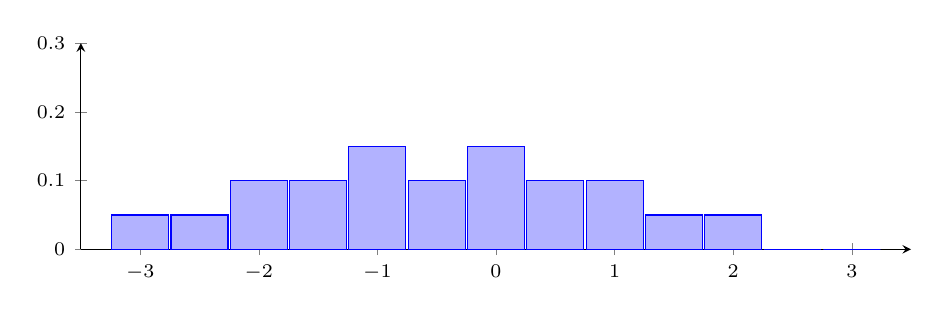
\begin{tikzpicture}
		\begin{axis}[
			width=\linewidth,
			height=4.2cm,
			ybar,
			bar width=0.48,
			xmin=-3.5,
			xmax=3.5,
			ymin=0,
			ymax=0.30,
			xtick={-3,-2,-1,0,1,2,3},
			ytick={0,0.1,0.2,0.3},
			yticklabels={0,0.1,0.2,0.3},
			axis lines=left,
			enlarge x limits=false,
			tick label style={font=\scriptsize},
			]
			\addplot coordinates {
				(-3,0.05)
				(-2.5,0.05)
				(-2,0.10)
				(-1.5,0.10)
				(-1,0.15)
				(-0.5,0.10)
				(0,0.15)
				(0.5,0.10)
				(1,0.10)
				(1.5,0.05)
				(2,0.05)
				(2.5,0)
				(3,0)
			};
		\end{axis}
	\end{tikzpicture}
}


\newcommand{\CSampleHistogramHundred}{
	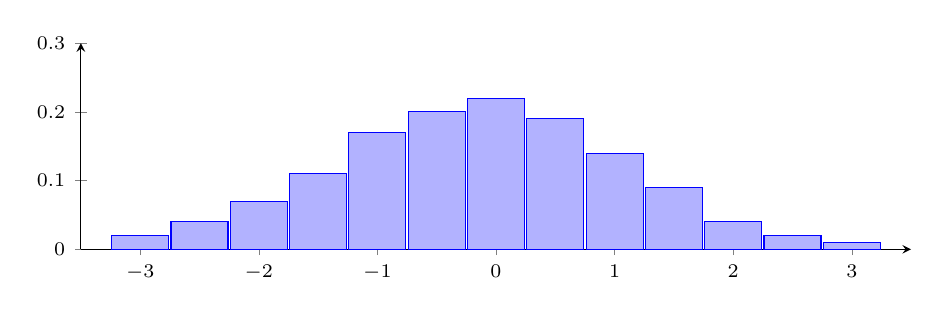
\begin{tikzpicture}
		\begin{axis}[
			width=\linewidth,
			height=4.2cm,
			ybar,
			bar width=0.48,
			xmin=-3.5,
			xmax=3.5,
			ymin=0,
			ymax=0.30,
			xtick={-3,-2,-1,0,1,2,3},
			ytick={0,0.1,0.2,0.3},
			yticklabels={0,0.1,0.2,0.3},
			axis lines=left,
			enlarge x limits=false,
			tick label style={font=\scriptsize},
			]
			\addplot coordinates {
				(-3,0.02)
				(-2.5,0.04)
				(-2,0.07)
				(-1.5,0.11)
				(-1,0.17)
				(-0.5,0.20)
				(0,0.22)
				(0.5,0.19)
				(1,0.14)
				(1.5,0.09)
				(2,0.04)
				(2.5,0.02)
				(3,0.01)
			};
		\end{axis}
	\end{tikzpicture}
}


\newcommand{\CSampleHistogramThousand}{
	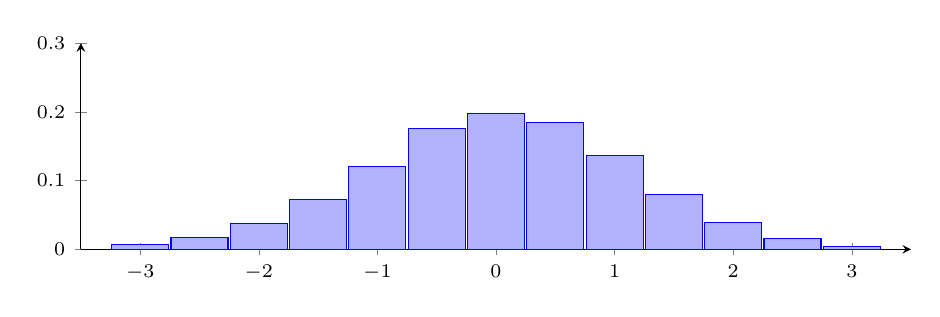
\begin{tikzpicture}
		\begin{axis}[
			width=\linewidth,
			height=4.2cm,
			ybar,
			bar width=0.48,
			xmin=-3.5,
			xmax=3.5,
			ymin=0,
			ymax=0.30,
			xtick={-3,-2,-1,0,1,2,3},
			ytick={0,0.1,0.2,0.3},
			yticklabels={0,0.1,0.2,0.3},
			axis lines=left,
			enlarge x limits=false,
			tick label style={font=\scriptsize},
			]
			\addplot coordinates {
				(-3,0.007)
				(-2.5,0.017)
				(-2,0.038)
				(-1.5,0.073)
				(-1,0.121)
				(-0.5,0.176)
				(0,0.198)
				(0.5,0.185)
				(1,0.137)
				(1.5,0.080)
				(2,0.039)
				(2.5,0.016)
				(3,0.004)
			};
		\end{axis}
	\end{tikzpicture}
}

\newcommand{\CSampleCountHistogramTwenty}{
	\begin{tikzpicture}
		\begin{axis}[
			width=\linewidth,
			height=4.2cm,
			ybar,
			bar width=0.48,
			xmin=-3.5,
			xmax=3.5,
			ymin=0,
			ymax=220,
			xtick={-3,-2,-1,0,1,2,3},
			ytick={0,50,100,150,200},
			axis lines=left,
			enlarge x limits=false,
			tick label style={font=\scriptsize},
			]
			\addplot coordinates {
				(-3,1)
				(-2.5,1)
				(-2,2)
				(-1.5,2)
				(-1,3)
				(-0.5,2)
				(0,3)
				(0.5,2)
				(1,2)
				(1.5,1)
				(2,1)
				(2.5,0)
				(3,0)
			};
		\end{axis}
	\end{tikzpicture}
}


\newcommand{\CSampleCountHistogramHundred}{
	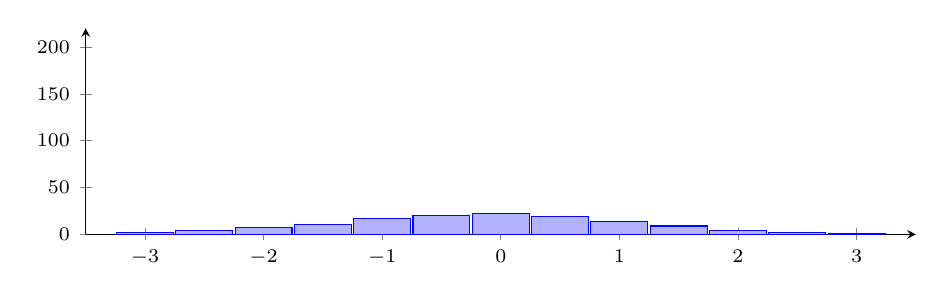
\begin{tikzpicture}
		\begin{axis}[
			width=\linewidth,
			height=4.2cm,
			ybar,
			bar width=0.48,
			xmin=-3.5,
			xmax=3.5,
			ymin=0,
			ymax=220,
			xtick={-3,-2,-1,0,1,2,3},
			ytick={0,50,100,150,200},
			axis lines=left,
			enlarge x limits=false,
			tick label style={font=\scriptsize},
			]
			\addplot coordinates {
				(-3,2)
				(-2.5,4)
				(-2,7)
				(-1.5,11)
				(-1,17)
				(-0.5,20)
				(0,22)
				(0.5,19)
				(1,14)
				(1.5,9)
				(2,4)
				(2.5,2)
				(3,1)
			};
		\end{axis}
	\end{tikzpicture}
}


\newcommand{\CSampleCountHistogramThousand}{
	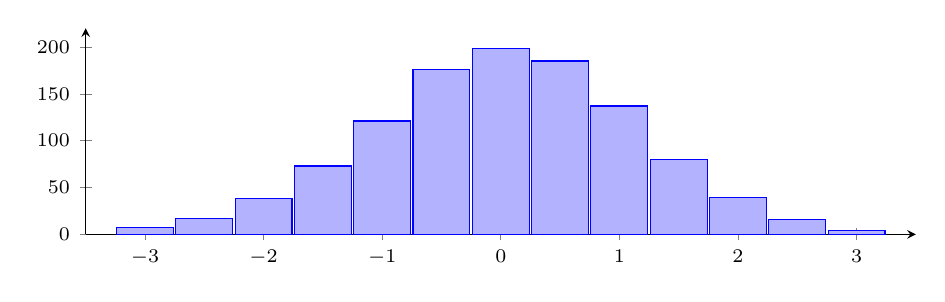
\begin{tikzpicture}
		\begin{axis}[
			width=\linewidth,
			height=4.2cm,
			ybar,
			bar width=0.48,
			xmin=-3.5,
			xmax=3.5,
			ymin=0,
			ymax=220,
			xtick={-3,-2,-1,0,1,2,3},
			ytick={0,50,100,150,200},
			axis lines=left,
			enlarge x limits=false,
			tick label style={font=\scriptsize},
			]
			\addplot coordinates {
				(-3,7)
				(-2.5,17)
				(-2,38)
				(-1.5,73)
				(-1,121)
				(-0.5,176)
				(0,198)
				(0.5,185)
				(1,137)
				(1.5,80)
				(2,39)
				(2.5,16)
				(3,4)
			};
		\end{axis}
	\end{tikzpicture}
}